\section{Ultrasonic Sensors}
The LIDAR [\ref{trm::LIDAR}] is a brilliant device, but due to the construction of the robot, a large section of the world cannot be scanned.
To combat this problem, several ultrasonic sensors are used, which function as sonar.

\subsection{Blind Spot}
As mentioned previously, the LIDAR is incapable of scanning in a roughly 100$^\circ$ arc.
This is due to the LIDAR being mounted on the front of the robot, and its line of sight is blocked behind it by the frame holding the laptop and the Raspberry Pis.
This is illustrated in figure \ref{fig::blindspot}.

\begin{figure}[H]
\centering
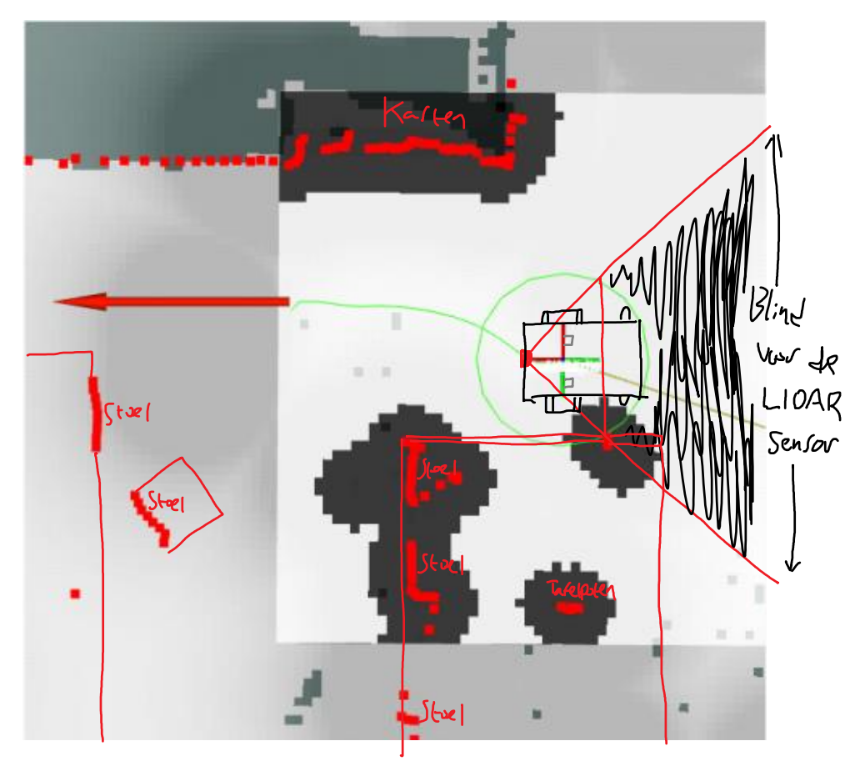
\includegraphics[width = 8cm]{WillyBlindSpot.PNG}
\caption{An illustration of the area WTR cannot see}
\label{fig::blindspot}
\end{figure}

The previous group managed to get WTR to the point where it can ignore its own frame as a potential obstacle through working with the AMCL.

As far as is known, there are currently no situations that would require WTR to reverse, since it will not reverse to reach a destination, but instead turn 180$^{\circ}$ and then drive forwards.
In addition, there are no known recovery behaviour patterns that would cause it to reverse either.
This means that there is no necessity to have vision, but for safety reasons the sides will still have to be checked.


\subsection{Sonar}
In order to make sure it cannot hit any people or object, two sonar sensors have been mounted on the sides just above the pivot wheels.
These have the fortunate benefit of not being based on light, and as such can detect glass or other transparent materials.
As such, more of these sensors are mounted on the front of WTR, to prevent collisions.
The current plan is to utilize these only for collision detection and leave them out of pathfinding calculations entirely, as they work a too short range to be used in long-distance planning.

When it comes to the recovery behaviours, the sonar sensors become very useful.
By default, the recovery behaviours do not include driving backwards at all, which is something good for WTR, since it is mostly blind as to what is going on behind it.
By using the sonar sensors to supercede the behaviour dictated by the ROS move\_ base, collisions can be avoided more easily.
When the recovery behaviours tell WTR to start spinning in place, the sonar sensors can tell WTR to stop moving immediately if something has moved near its rear.
An emergency signal can be sent to the move\_ base, at which point WTR can either wait or attempt a new behaviour in order to recover anyway.
If it was turning left for example, it can try moving right instead.
\newpage
